\documentclass[12pt]{article}
\usepackage{amsmath}
\usepackage{amsfonts}
\usepackage{amssymb}
\usepackage{subfig}
\usepackage{graphicx}
\usepackage{float}
%\usepackage[cm]{fullpage}


%%%%% TIKZ CODE (For Feynman diagrams)
\usepackage{tikz}
\usetikzlibrary{arrows,shapes}
\usetikzlibrary{trees}
\usetikzlibrary{matrix,arrows} 				% For commutative diagram
											% http://www.felixl.de/commu.pdf
\usetikzlibrary{positioning}				% For "above of=" commands
\usetikzlibrary{calc,through}				% For coordinates
\usetikzlibrary{decorations.pathreplacing}  % For curly braces
\usetikzlibrary{backgrounds}  				% For showing background grid
\usepackage{pgffor}							% For repeating patterns

\usetikzlibrary{decorations.pathmorphing}	% For Feynman Diagrams
\usetikzlibrary{decorations.markings}
\usetikzlibrary{snakes}
\tikzset{
	% >=stealth', %% Different kind of arrows
    vector/.style={decorate, decoration={snake}, draw},
    fermion/.style={draw=black, postaction={decorate},
        decoration={markings,mark=at position .55 with {\arrow[draw=black]{>}}}},
    fermionbar/.style={draw=black, postaction={decorate},
        decoration={markings,mark=at position .55 with {\arrow[draw=black]{<}}}},
    fermionnoarrow/.style={draw=black},
    gluon/.style={decorate, draw=
        decoration={coil,amplitude=4pt, segment length=5pt}},
    scalar/.style={dashed,draw=black, postaction={decorate},
        decoration={markings,mark=at position .55 with {\arrow[draw=black]{>}}}},
    scalarbar/.style={dashed,draw=black, postaction={decorate},
        decoration={markings,mark=at position .55 with {\arrow[draw=black]{<}}}},
    scalarnoarrow/.style={dashed,draw=black},
%
%% 	Special vectors (when you need to fine-tune wiggles)
	provector/.style={decorate, decoration={snake,amplitude=2.5pt}, draw},
	antivector/.style={decorate, decoration={snake,amplitude=-2.5pt}, draw},
}



\textwidth 6.5in
\oddsidemargin 0in
\evensidemargin 0in
\textheight 8.6in
\topmargin -0.5in
\pagestyle{empty}
\begin{document}

\vspace*{-1cm}
\begin{center}
{\LARGE \bf Relativistic Quantum Field Theory}

\vspace*{0.5cm}
{\Large Physics 7651} \\
\vspace*{0.5cm}
{\Large {\bf Homework 7}\\
\vspace*{0.5cm}
Due: In class on Wednesday, October 19}
\end{center}
\begin{enumerate}



\item {\bf Some cross section calculations} [5 points]

Here we will the theory in Problem 1 of Homework 6 to experimental observables. Recall that the Lagrangian of that theory was
$$
\mathcal L = \frac 12 \left(\partial \phi\right)^2  - \frac 12 m^2\phi^2 + \left|\partial \psi\right|^2 - M^2 |\psi|^2 - g\phi\psi^\dagger\psi.
$$
\begin{enumerate}
\item Compute, to leading order in $g$, the center-of-mass differential cross section and total cross section for the elastic scattering of $\psi\psi^\dag$.
\item Do the same for $\psi\psi^\dag$ annihilating into $\phi\phi$. \textit{Hint:} you already calculated the amplitude in Homework 6. Be careful not to double-count final states.
\item Do the same for $\psi\phi \to \psi \phi$. \textit{Hint:} you calculated the amplitude in  Homework 6.
\end{enumerate}

\vspace{1em}

\item {\bf Kinematics of a simple theory} [10 points]

\begin{enumerate}
\item Work out the three-body phase space $D_{(3)}$ for massless final states. Explicitly give the integration range for $dE_1\, dE_2$. Draw the Dalitz plot for this process.

\item Let $A$, $B$, $C$, and $D$ be four real scalar fields with Lagrangian
$$\mathcal L = \frac 12 \left[
(\partial A)^2 - m^2 A^2
+ (\partial B)^2
+ (\partial C)^2
+ (\partial D)^2
\right]
+ g ABCD.
$$
Compute, to the lowest non-vanishing order in $g$, the total decay width of the $A$. How would the answer have differed if the interaction were instead $gAB^3$?

\end{enumerate}


\vspace{1em}

\item{\bf Particle decay in a thermal universe} [5 points]

Consider a theory in which a heavy real scalar $\varphi$ can decay into ligher real scalars  $\phi$. The particular interaction is not relevant. Thus far we have studied such a decay with the implicit assumption that the universe was empty of $\phi$ particles before the decay. Sometimes (e.g.\ in cosmology) we would like to compute the decay of a $\varphi$ not in an empty universe, but one that was already filled with a thermal distribution of $\phi$ particles. 

This is not hard to do if you treat the final state particles as non-interacting and assume that there are no other $\varphi$ type particles in the initial distribution of particles\footnote{This frequently happens in cosmology: the $\varphi$ may be heavy and produced in thermal equilibrium at an early epoch when the temperature was very high. The expansion of the universe rapidly brings these particles out of equilibrium (`freeze out') and reduces their density to a negligible value. They then decay in an environment consisting of a hot gas of the much less massive $\phi$ particles.}.


Show that in this case the only change in the formalism presented in class is that the phase space density $D$ has an additional multiplicative factor $f(E/k_BT)$ for reach final state $\phi$, where $E$ is the $\phi$ energy, $k_B$ is Boltzmann's constant, and $f$ is a function that you must find.

\textit{Hints:} (1) For any system in thermal equilibrium, the probability of finding a system in its $n^\text{th}$ energy eigenstate is proportional to $\exp(-E_n/k_BT)$. (2) For a single harmonic oscillator, $\langle n | a^\dag | n-1 \rangle = \sqrt{n}$.


\vspace{1em}

\item{\bf Introduction to scalar QED} [10 points]

We have referred to the conserved charge of a complex scalar field $\psi$ as its electric charge. In this problem we will see how this is done by introducing a photon, $A_\mu$ which couples to this charge. The photon is a vector particle (you can think of it as the quantized vector potential), which is something we haven't seen before. We'll meet the photon later in this course and delve further into gauge theories next semester; for now we'll just get our feet wet.

One might like to couple the photon directly to the Noether current as $\mathcal L_I = -j^\mu A^\mu$, but this is not gauge invariant. The correct Lagrangian for scalar QED is obtained through minimal coupling and is
$$ 
\mathcal L = -\frac{1}{4}F_{\mu\nu}F^{\mu \nu}
+ (D_\mu \psi)^\dag D^\mu \psi - m^2 |\psi|^2,
\qquad\qquad
D_\mu = \partial_\mu + ieA_\mu,
$$
where the $F^2$ term is the photon kinetic term and $e$ is the electric coupling. 

\begin{enumerate}
\item Write out the Feynman rule for the coupling between a charged scalar, its antiparticle, and the $\mu^\text{th}$ component of the photon assuming all momenta flowing into the vetex. Draw a charged particle as a line with an arrow and the photon as a wiggly line. 
%
\textit{Hint}: this is a derivative coupling. You learned how to deal with this in Problem 4 of HW6 so that you can `read off' the Feynman rule from the interaction Lagrangian\footnote{See Preskill 4.33 for a discussion of subtleties. If you are particularly conerned about formalities, you may simply take $H_I = -L_I$ and assume that $\partial_0$ commutes with time ordering.}. 
%Ignore the subtleties of $H_I$ not being Lorentz covariant. Instead, identify $H_I=-\mathcal L_I$ and assume that you can use Wick's theorem to turn the time ordering into normal ordering without worrying about $\partial_0$ terms\footnote{This ends up giving the correct rule since two subtleties cancel. See Preskill 4.33 for a discussion.}. 
\item The propagator for a photon in Feynman gauge is
$$
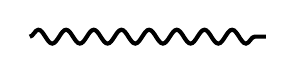
\begin{tikzpicture}[scale=1.5, line width=1.5pt]
	\draw[vector] (0,0) -- (2,0);
\end{tikzpicture}
= \frac{-ig_{\mu \nu}}{p^2 + i\epsilon}.
$$
Calculate the differential cross section $d\sigma/d\cos\theta$ for elastic $\psi \psi^\dag$ scattering.
\end{enumerate}




\end{enumerate}

\end{document}
